\documentclass[a4paper, 11pt]{article}

\usepackage{amsmath}
\usepackage{amssymb}
\usepackage{hyperref}
\usepackage{makeidx}
\usepackage{graphicx}
\usepackage{titlesec}
\titlespacing{\section}{0pt}{\parskip}{-\parskip}
\titlespacing{\subsection}{0pt}{\parskip}{-\parskip}
\graphicspath{{figures/}} % Directory in which figures are stored
\usepackage{natbib}% \bibliography
\usepackage{float}
\usepackage{setspace} % for line spacing
\usepackage[margin=1in]{geometry}
\title{Assignment4 Feature selection-CSE780}
\author{Paria, Fakhrzad \\ Stuent ID: 400353290 }
\date{21-Nov-2021}
\setstretch{1.3}
\setlength\abovecaptionskip{-5pt}

\begin{document}
	\maketitle
	\newpage
\section*{Part a. Data}
Nowadays having property insurance is one of the most important sections in people life. One of insurance contracts is related  to cars. In this report we will use a dataset related to an insurance company \cite{Kaggle}. There are 10000 customers in this data. Also there are 17features.The response column is a binomial factor variable that shows whether customer had insurance claim last year or not. We will see that how with these features to predict the customer behavior in claiming the insurance for accidents.\newline
There are 1939 NA observations in dataset that all have removed.\newline
\section*{Part b. Spars and non-spars models}
In this report, we will discuss the result of fitting three models 1)Ridge regression,  2)LASSO,  3)PLS and also will use best subset selection algorithm for choosing the best predictors that have relevant to our prediction.
These models have been choosen because all of them help us to find the most significant features that can explain the response. The comparison metric in this report is train MSE and accuracy percentage of test prediction.
 
Before fitting models to our dataset, since we have factor and categorical features, so we convert them to dummy features for better prediction. So the number of features will be 24 after this transformation. Also regarding features are measured in different scales we standardize the dataset with mean of zero and standard deviation 1.
We split the observations to train(50\%) and test(50\%) to estimate the test error.
\newline
\subsection*{b.1 Ridge Regression}
In ridge regression model we will have all the predictors/features in our model and as can seed in figure1 the number of features is 24.  We need to specify the optimal tuning parameter $\lambda$ and here we used cross validation in the train part of our dataset. The best $\lambda$ is 0.01. Then we predict with the test part of our dataset and we can see that MSE=0.268 and accuracy based on confusion matrix is 57\%. In tabel1 we see the lowest regression coefficient for ridge regression that as our expectation, non of them are zero.

\begin{table}[ht]
	\centering
	\caption{Feature Coefficient}
	\label{table1}
	\begin{tabular}{c|r}
		\hline
		Feature & Ridge Regression \\ 
		\hline
		raceminority  & -0.0028 \\ 
		educationuniversity & 0.0016  \\ 
		educationnone       & -0.0016 \\ 
		credit\_score     & -0.0022 \\  
		\hline
	\end{tabular}
	\quad
		\begin{tabular}{c|r}
		\hline
		Feature & LASSO \\ 
		\hline
		raceminority  & 0 \\ 
		educationuniversity & 0  \\ 
		educationnone       & 0 \\ 
		credit\_score     & 0.0014 \\  
		\hline
	\end{tabular}
\end{table}

\begin{figure}[H]
	\centering
	\begin{minipage}[b]{0.4\textwidth}
	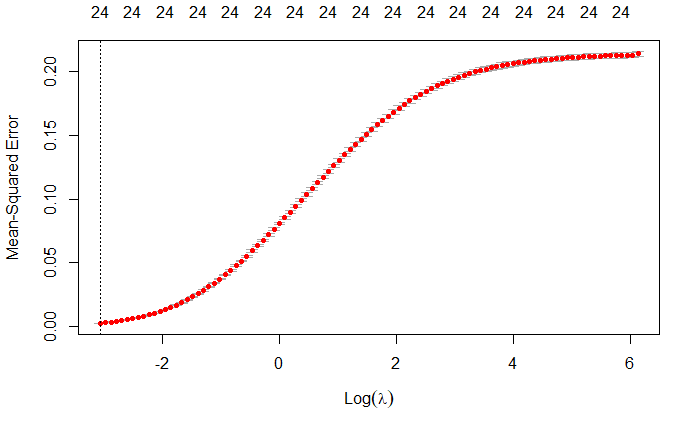
\includegraphics[width=\textwidth]{figure1.png}
	\caption{MSE and Lambda under Ridge regression }
\end{minipage}
	\begin{minipage}[b]{0.4\textwidth}
	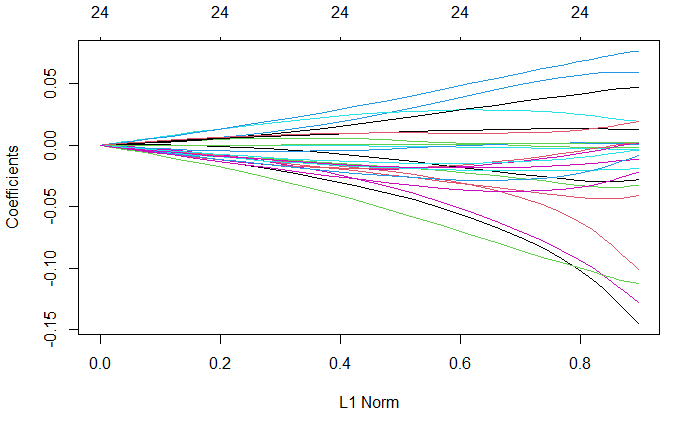
\includegraphics[width=\textwidth]{figure3.png}
	\caption{Coefficient under Ridge regression }
\end{minipage}
\end{figure}

\subsection*{b.2 LASSO }
We fit lasso model for the same train data and in figure 2 shows that in this model some of coefficient would be zero. The best $\lambda$ in this model is 0.001 and MSE=0.267, Accuracy is 57\%. 
\begin{figure}[H]
\centering
\begin{minipage}[b]{0.4\textwidth}
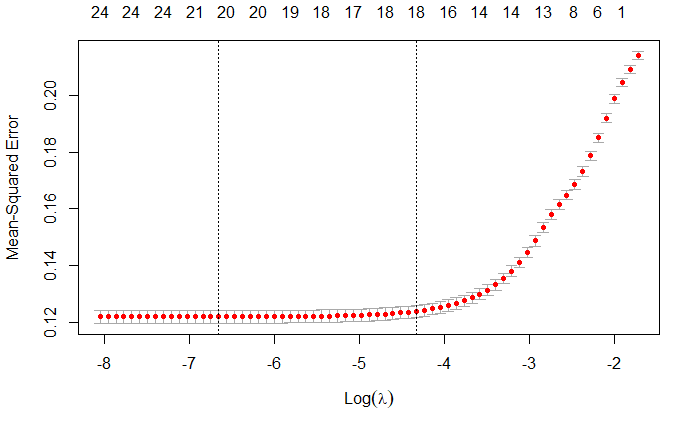
\includegraphics[width=\textwidth]{figure4.png}
\caption{MSE and Lambda under LASSO }
\end{minipage}
\begin{minipage}[b]{0.4\textwidth}
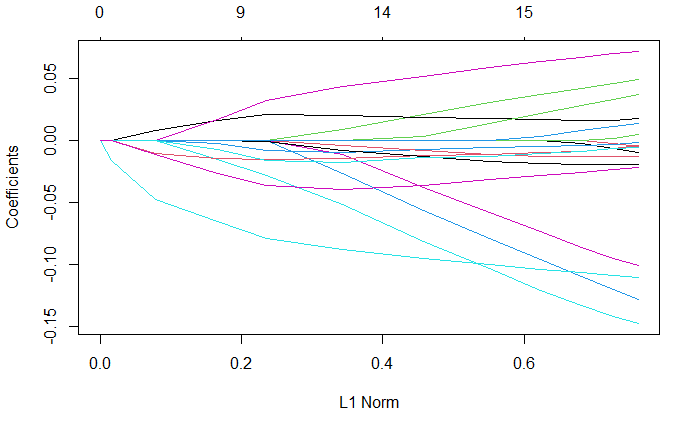
\includegraphics[width=\textwidth]{figure2.png}
\caption{coefficient and Lambda under LASSO }
\end{minipage}
\end{figure}

\subsection*{b.3 Partial Least Square PLS }
With fitting PLS in this dataset we can see in figure6 that CV error minimized at component=3. When we predict the response with test data, can see than the accuracy is 93\% and MSE=0.12.\newline

\subsection*{b.4 Best subset selection }
With performing the best subset selection in this dataset we will see that DUI, raceminority, educationnone, educationuniversity, incomeupper class,credit\_score and speeding\_violations have the least effect in selecting different models and with comparing to Tabel1 , somehow we can see that the features with zero coefficient are in this list. Based on adjusted $R^2$ in feature5, the number of features selected 17 from 24.

\begin{figure}[H]
	\centering
	\begin{minipage}[b]{0.4\textwidth}
		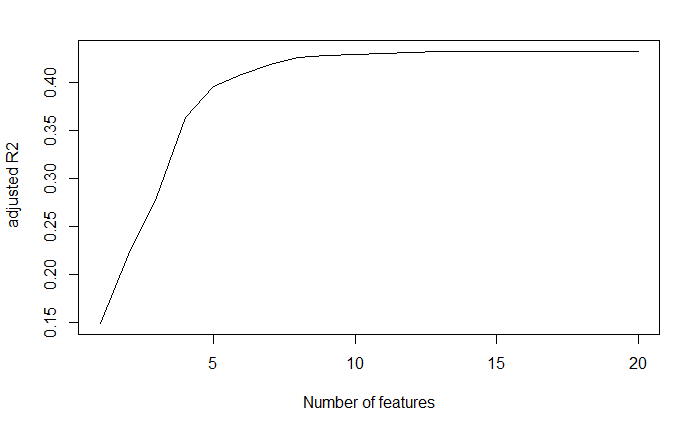
\includegraphics[width=\textwidth]{figure5.png}
		\caption{$R^2$ and number of features under best subset selection }
	\end{minipage}
	\begin{minipage}[b]{0.4\textwidth}
		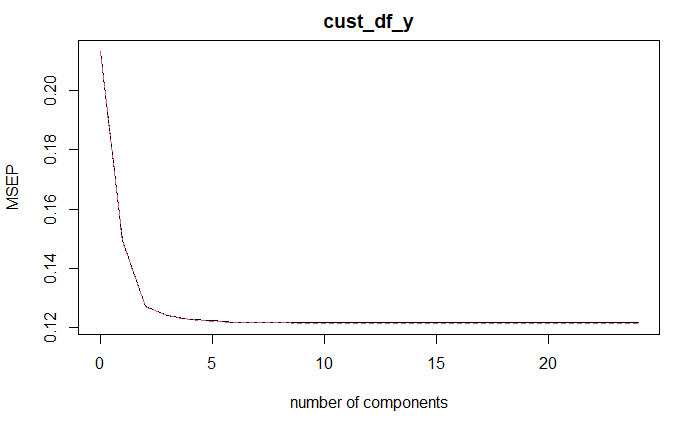
\includegraphics[width=\textwidth]{figure6.png}
		\caption{ optimal number of components under PLS }
	\end{minipage}
\end{figure}

\section*{Part c. Result }
As we can see in tables1, features which in ridge regression had very small coefficient in the best $\lambda$ in RASSO their coefficients are zero. Also and comparison in tabel2, the accuracy in RASSO is better than ridge regression. The result shows that the most accurate model in this case in PLS, since it uses the label for feature extraction also in this model all features will be used for forming the first three components and here we can conclude that there are small collinearity between features.
 
\begin{table}[ht]
	\centering
	\caption{Models comparison}
	\label{table2}
	\begin{tabular}{clrr}
		\hline
		\textbf{Model} & \textbf{Type} & \textbf{Test MSE} & \textbf{Test Accuracy} \\ 
		\hline
		\textbf{Ridge regression}  & non-sparse & 0.267 & 55\% \\ 
		\textbf{LASSO} & sparse & 0.267 & 57\% \\ 
		\textbf{PLS}   & feature extraction & 0.127 & 92\% \\   
		\hline
	\end{tabular}
\end{table}
\newpage
\bibliographystyle{plain}
\bibliography{Assignment4}
\end{document}
